\section{Comparison To Previous Model}
\label{ch:AmareshComparison}

\begin{frame}
\frametitle{Comparison Between Old and New Profiles}

\begin{columns}[onlytextwidth]
  \begin{column}{0.5\textwidth}
    \begin{itemize}
			\item While both distributions have approximately the same width (after
      scale-factor is applied), the internal structure is quite different.
      \item Notably, the simple profile model is extremely asymmetric.
			\item Additionally, the tails in the realistic profile are more
				significant.
			\item Note that normalization between the profiles is applied
				differently.
    \end{itemize}
  \end{column}

  \begin{column}{0.5\textwidth}
    \centering
    \begin{figure}
    \begin{center}
    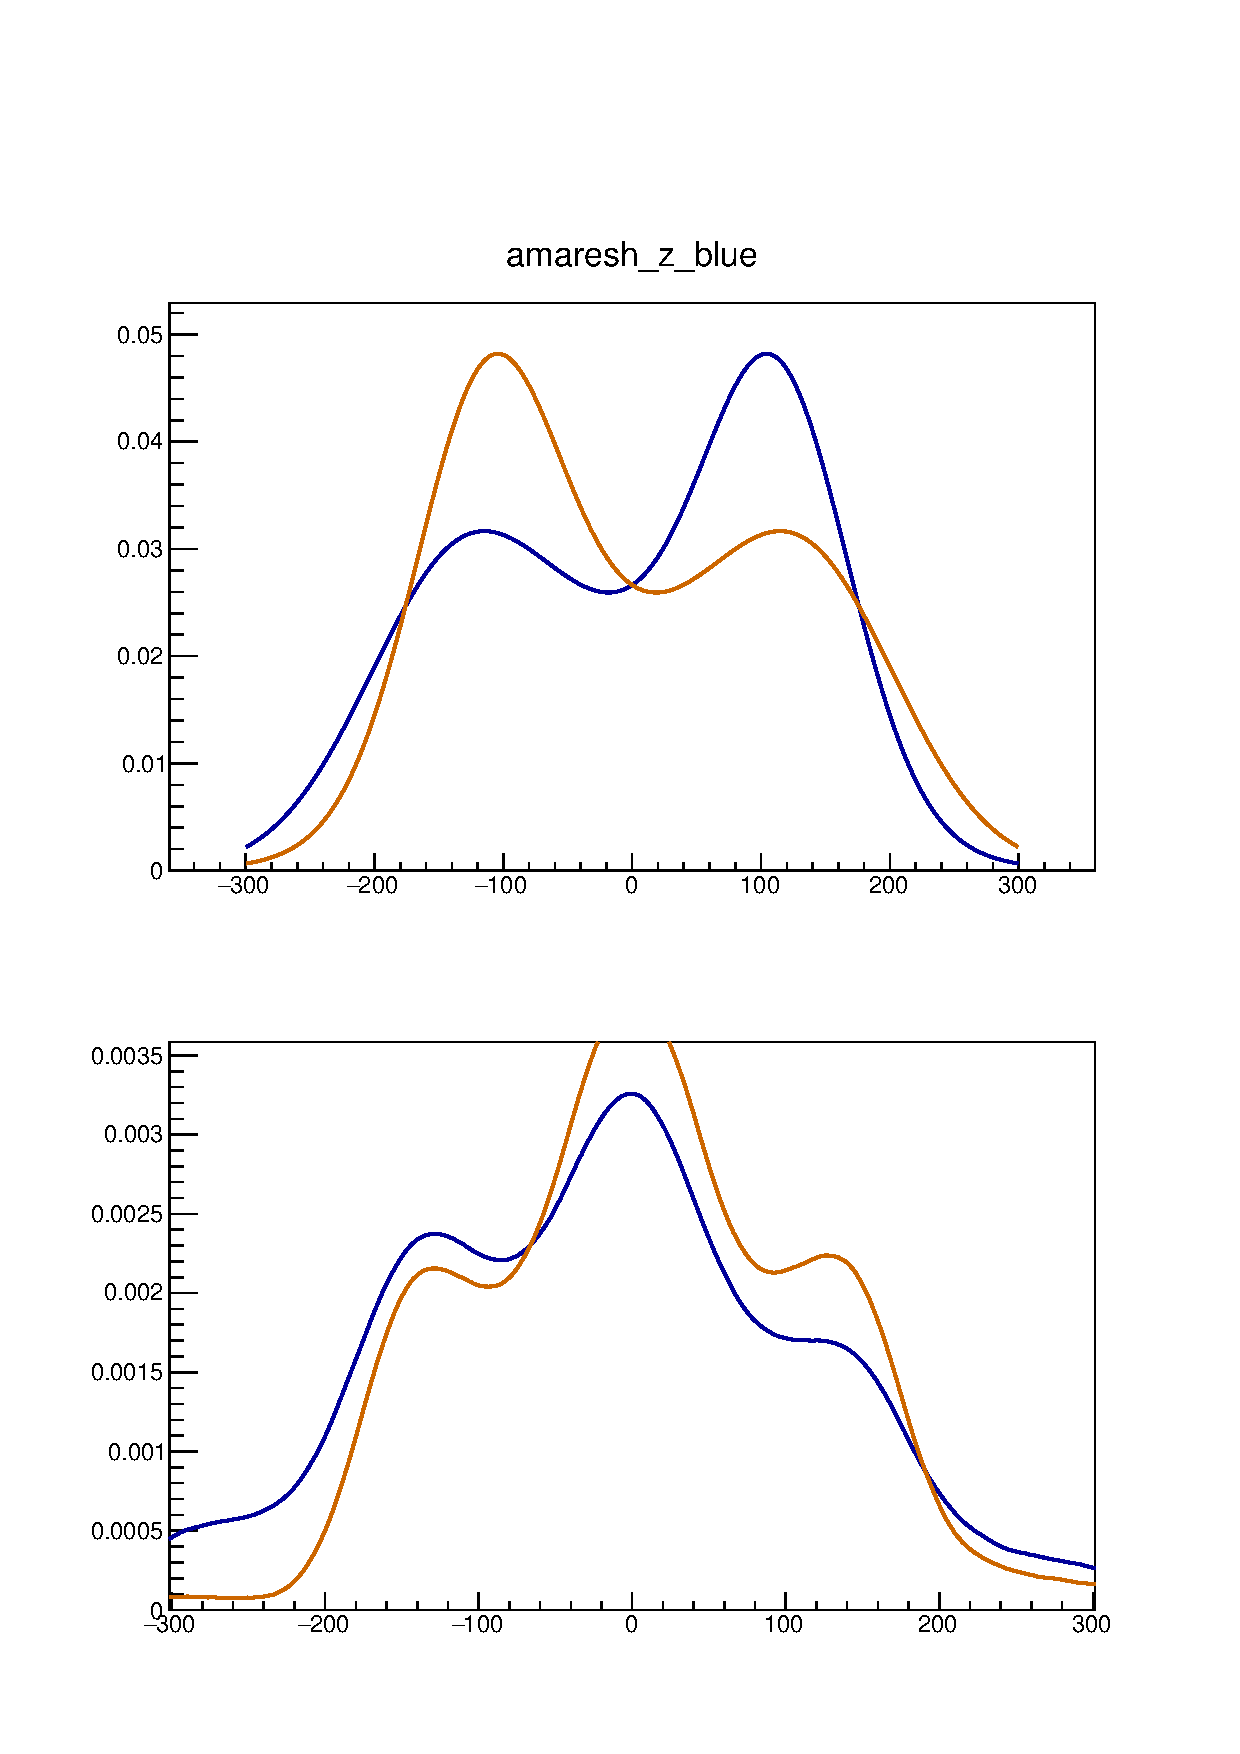
\includegraphics[width=0.8\linewidth]{../AmareshComparison/figs/z_prof_comparison.pdf}
    \end{center}
    \caption{Bottom: the "real" profile, Top: the "simple" profile used in other analyses.}
    \label{fig:z_prof_comparison_amaresh_new}
    \end{figure}
  \end{column}
\end{columns}
\end{frame}

